\chapter{АНАЛИЗ ПРОГРАММНОГО ОБЕСПЕЧЕНИЯ ДЛЯ ПРОГРАММИРОВАНИЯ И РАЗРАБОТКИ РОБОТОТЕХНИЧЕСКИХ СИСТЕМ}

В первом разделе данной главы производится обзор фрэймворка робота. Весь API подробно рассматриваться не будет в связи с тем, что все управление роботом в дальнейшем будет производиться через методы классов, предоставляемых симулятором Webots. Взаимодействие с интерфейсом DARwIn Framework будет происходить только при компиляции модуля для интерпретации движений непосредственно на самом роботе. Это связано с тем, что вызовы методов классов Webots для управления моторами на физической модели робота имеют существенные задержки во времени, которые не позволяют роботу совершать плавные и непрерывные движения.

Так же кратко был рассмотрен интерфейс управления приводами одного из самых распространенных гуманоидных роботов Nao. Этот анализ был произведен для получения представления о имеющихся аналогах систем управления: их плюсах и недостатках.

Далее, исходя из ранее полученных знаний, был разработан интерфейс класса для языка программирования C++. Другие популярные языки высокого уровня, такие как Java и Python, были исключены из-за их низкой производительности. Для поддержки данных языков в реализованного модуля управления можно воспользоваться инструментом связывания программ и библиотек, написанных на языке C и C++, с интерпретируемыми (Tcl, Perl, Python, Ruby, PHP) или компилируемыми (Java, C\#, Scheme, OCaml) языками - SWIG\cite{beazley1997swig}.


\section{Анализ DARwIn Framework}

В данном разделе будет произведет поверхностный обзор системы управления роботом, предоставляемого разработчиками платформы. Подробной документации о библиотеке производитель не распространяет.

Исходный код фреймфорка, написанного на языке C/C++, для платформы DARwIn-OP можно получить из репозитория проекта на сайте SourceForge. Так же используемые в данной работе классы доступны в пакете симуляции Webots в каталоге с модулями для данного робота. Симуляционная среда будет подробнее рассматриваться в следующем разделе.

Ниже приведена диаграмма классов (Рис. \ref{im:1_framework_class_diagram}), доступная в официальной документации\cite{urldarwinopemanual}. На данной диаграмме отображены все основные классы, которые используются при взаимодействии с роботом.

\begin{figure}[h]
\center{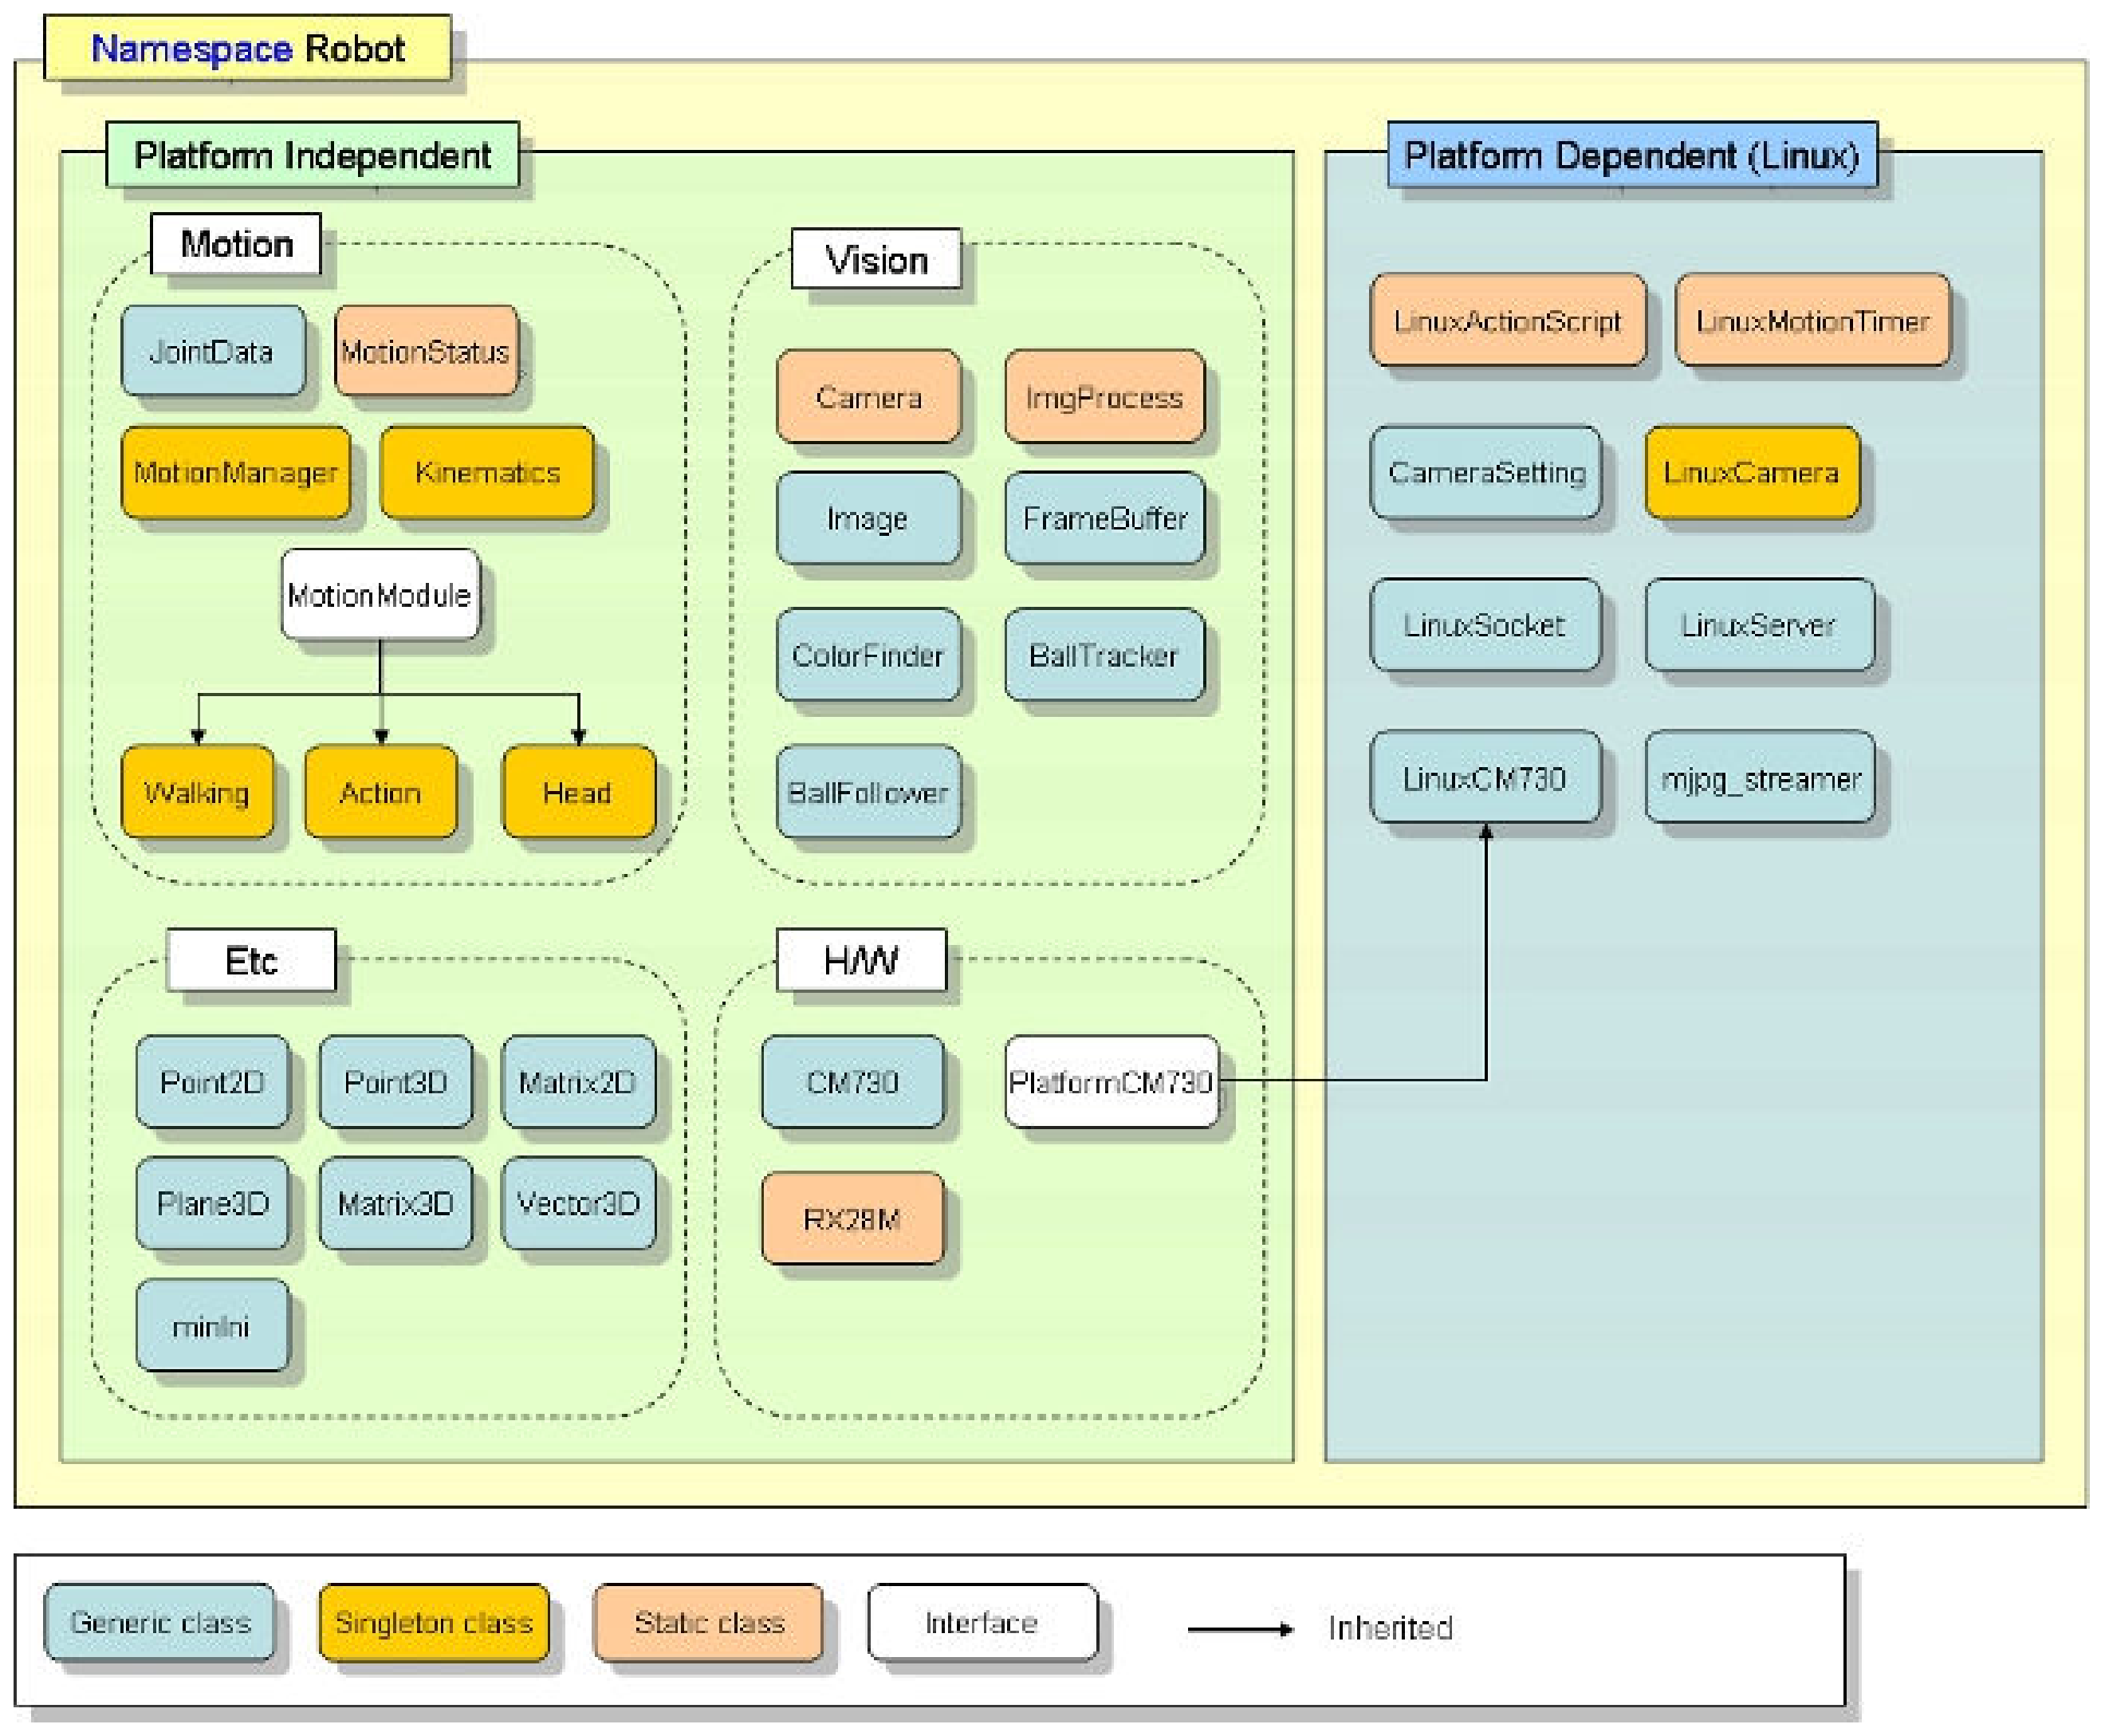
\includegraphics[width=1\linewidth]{1_framework_class_diagram}}
\caption{Диаграмма классов DARwIn Framework.}
\label{im:1_framework_class_diagram}
\end{figure}

Все классы находятся в области видимости Robot и делятся на платформонезависимые элементы и элементы, написанные для операционной системы Linux. Сам робот работает под управлением операционной системы Linux Ubuntu 9.10. Из данных классов интерес предоставляют элементы групп H/W и Motion.

Класс CM730 отвечает за взаимодействие программы-контроллера с субконтроллером робота. Класс CM730 предоставляет возможность получать информацию с устройств, подключенных к данной плате (гироскоп, акселерометр, кнопки, сервоприводы и т.д.), а так же отправлять данные на светодиодные индикаторы и сервоприводы. Отправка и получение данных с соответствующих устройств происходит с задержкой в 1 мс. Для увеличения производительности умправление моторами робота происходит единым пакетом данных c задержкой 1-2 мс \cite{mansolino2013robot}.

Для управления движениями робота была реализована группа классов Motion. Класс JointData является контейнером данных для взаимодействия с моторами робота. Он хранит данные PID-контроллера  и позиции для каждого сервопривода, а так же предоставляет публичные методы для взаимодействия с этими переменными.

Класс Kinematics имеет статические поля с информацией о длинах составляющих ноги робота (высота бедра, голени и стопы) и информацию о позиции камеры. Информации о длинах составляющих рук в данном классе отсутствует и была получена из документации о кинематике робота \cite{williams2012darwin}.

MotionModule является интерфейсом для управления движениями робота. Данный интерфейс хранит экземпляр JointData для взаимодействия алгоритма с моторами. Производитель робота предоставляет в данном фреймворке готовый модуль управления походкой робота (Walking), модуль воспроизведения записанных движений (Action) и модуль для управления головой робота (Head).

Подробнее рассматривается реализация модуля походки робота. Параметры походки читаются из конфигурационного *.ini файла с помощью библиотеки miniIni, которая идет в комплекте с данным фреймворком. Далее приведены основные параметры, которые описываются в файле: начальное смещение стопы по оси X в миллиметрах, начальное смещение стопы по оси Y в миллиметрах, начальное смещение стопы по оси Z в миллиметрах, начальный разворот стопы вокруг оси X в градусах, начальный разворот стопы вокруг оси Y в градусах, начальный разворот стопы вокруг оси Z в градусах, угол наклона туловища в градусах, период двух шагов в миллисекундах, соотношение времени между периодом переноса ноги и остановки, длина шага в миллиметрах, максимальная амплитуда поднятия стопы в миллиметрах, амплитуда смещения туловища влево-вправо в миллиметрах, амплитуда подъема-опускания туловища в миллиметрах. Данный перечень параметров можно сгруппировать в параметры положения и вращения туловища и параметры положения и вращения левой и правой стопы, что необходимо для дальнейшей разработки системы управления роботом. Сам алгоритм походки состоит из поочередного переноса стопы по синусоидальной траектории: высчитывается позиция стопы в каждый момент времени и решается задача обратной кинематики для расчета позиций моторов. Так же стоит обратить внимание, что алгоритм реализован некорректно при развороте стопы вокруг оси Z и ненулевом наклоне туловища: наклон робота происходит путем добавления угла наклона к позиции моторов бедер, а при вращении ноги вокруг оси Z данный угол должен был распределяться на два мотора на каждой ноге. В разработке системы управления механикой этот фактор так же был учтен.

Статический класс MotionStatus является контейнером для данных, полученных с гироскопа, акселерометра и кнопок робота.

Класс MotionManager является связующим звеном между реализациями MotionModule и MotionStatus с классом CM730: класс передает данные из активных модулей движения непосредственно на физические моторы.
Для демонстрации взаимодействия классов ниже приведена схема передачи данных между модулями робота (Рис. \ref{im:1_framework_pipeline}), доступная в официальной документации робота\cite{urldarwinopemanual}.

\begin{figure}[h]
\center{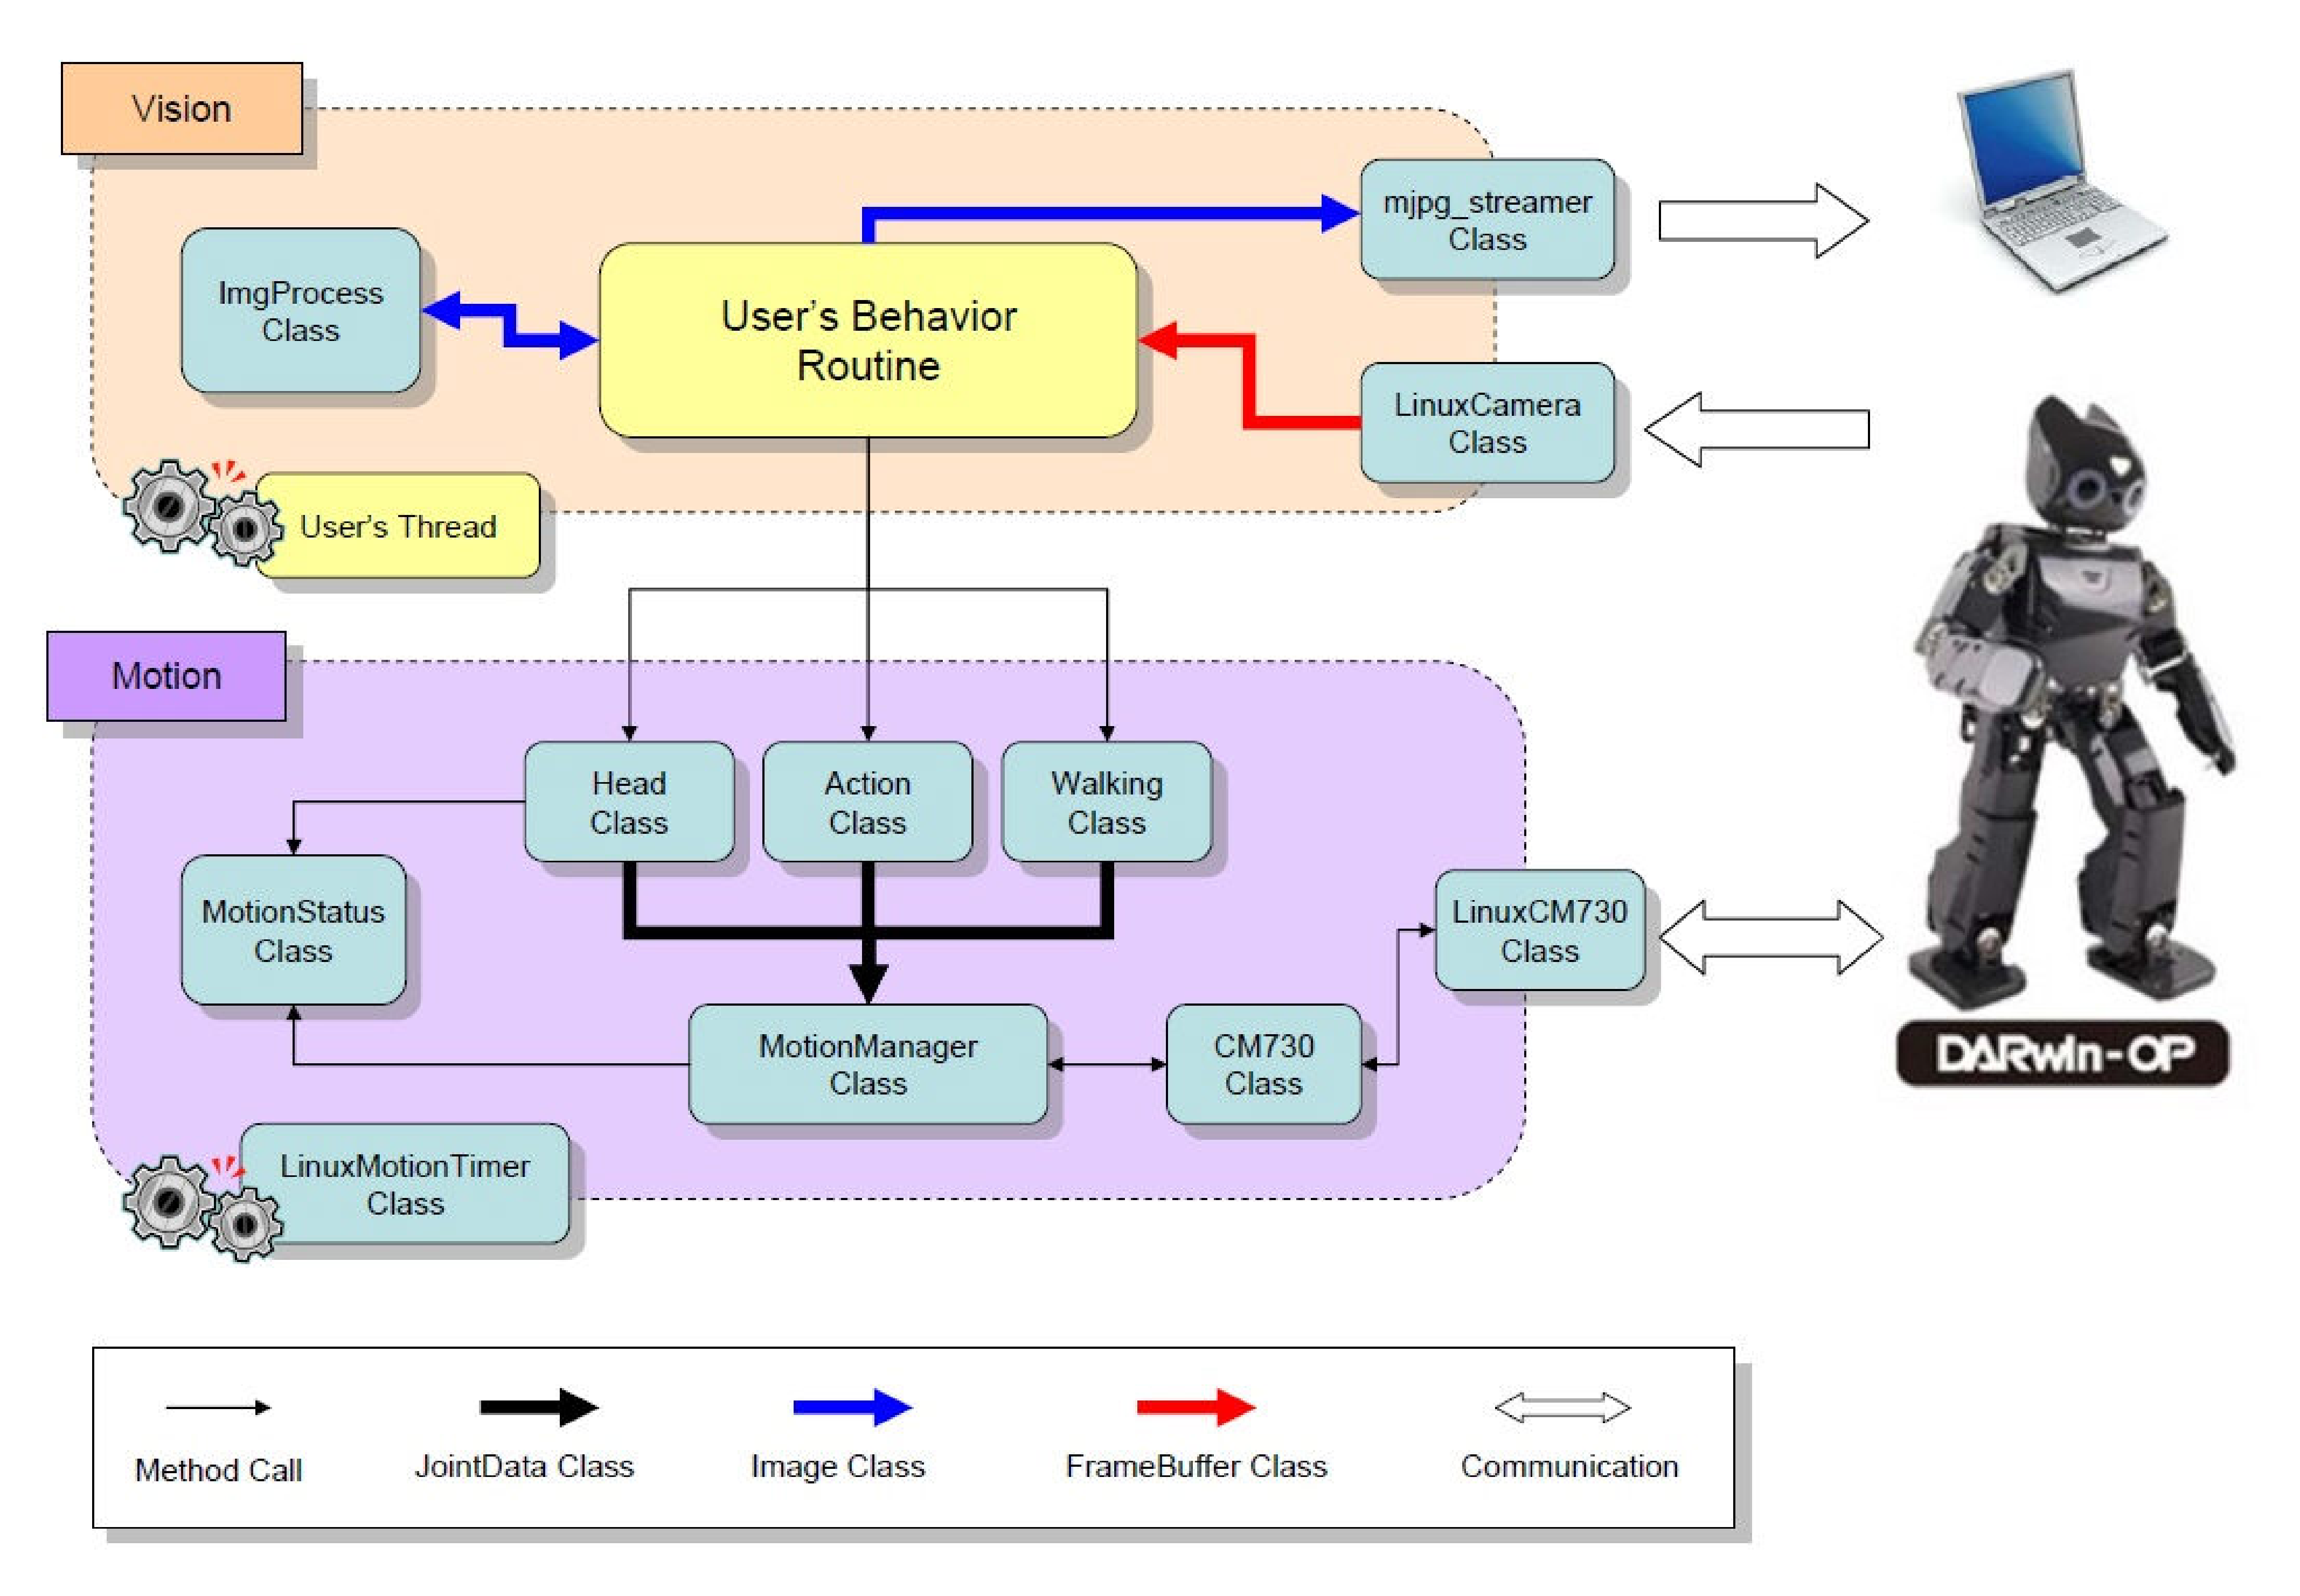
\includegraphics[width=1\linewidth]{1_framework_pipeline}}
\caption{Диаграмма передачи данных между модулями робота.}
\label{im:1_framework_pipeline}
\end{figure}

Необходимо заметить, что в фрэймворке отсутствует готовая реализация механизма программным управлением движений с помощью перемещений декартовой системы координат. Исходя из этого можно утверждать, что возможность выполнения движения удара ногой при использовании стандартного функционала у данного робота ограничивается механизмом воспроизведения записанных движений и отсутствует возможность динамеческого управления траектории удара, например, при игре футбол.

Обобщив выше сказанное, Darwin Framework предоставляет собой полноценный низкоуровневый компонент для управления роботом. Исходные коды находятся в открытом доступе. Это позволило обнаружить ошибки, допущенные в нем (описание ошибки в классе Walk представлено в этом разделе). В пакете разработки отсутствуют высокоуровневые механизмы взаимодействия с роботом и это является основной причиной, из-за чего в ходе данной работы разрабатываются библиотека управления.

\section{Анализ симуляционной среды Webots}

Для возможности программно симулировать поведение робота был выбран кросплатформенный робототехнический симулятор Webots 8.0. В данном симуляторе имеется полная поддержка DARwIn-OP, за исключением возможности воспроизведения звука. Так же симулятор позволяет запускать и тестировать код непосредственно на самом роботе.

В данном разделе описаны базовые классы, входящих в состав Webots, для программирования робота Darwin-OP и основные возможности симулятора. Подробное описание возможностей симулятора выходит за пределы данной работы. 

Перед тем, как начать рассмотрение базовых классов, предоставляемых симулятором для взаимодействия роботом, стоит упомянут о различии процесса компиляции программного контроллера (программы управления роботом) под симулятор и для компиляции контроллера на реальном роботе. Симулятор Webots предоставляет разработчику набор абстрактных классов для взаимодействия с роботом. Компиляция для запуска программы на реальном роботе происходит с ключом -DCROSSCOMPILATION для компилятора gcc. Другими словами этот ключ объявляет макрос C/C++ при сборке всего исходного кода. С помощью механизма макроподстановки в языке данный ключ сообщает о том, нужно ли использовать механизмы управления, предоставляемые Darwin Framework, или контроллер будет использовать классы для поддержки симуляции в среде Webots. Контроллер, собранный с поддержкой симуляции, нельзя запустить на роботе и так же нет возможности запустить контроллер, собранный для робота, в симуляторе.

Далее приведено описание базового набора классов управления роботом. Эти классы были использованы в ходе разработки собственного программного компонента управления.

При компиляции контроллера для запуска на роботе все перечисленные классы являются оберткой вокруг вызовов методов классов Darwin Framework.

Ключевым классом контроллера является класс Robot. Класс пользовательского контроллера обязательно должен быть наследован от данного класса. В нем происходит инициализация оборудования и основных механизмов, а так же происходит обновление данных устройств. Для робота заданы хэш-таблицы с существующим набором светодиодных индикаторов, сервоприводов, позиционных сенсоров, гироскопа, акселерометра и кнопок. Для поддержки пошаговой симуляции в классе определен метод int step(time\_step). Данный метод должен вызываться на каждой итерации работы контроллера для обновления данных и взаимодействия с симулятором.

Класс Accelerometer отвечает за работу акселерометра. Класс возвращает целочисленное значение от 0 до 1024, что соответствует диапазону значений от -3$g$ до 3$g$.

Класс Gyro отвечает за работу гироскопа. Класс возвращает целочисленное значение от 0 до 1024, что соответствует диапазону значений от -160 град/сек до 160 град/сек.

Для взаимодействия с сервоприводами в симуляционной среде существуют два класса: PositionSensor и Motor. Первый класс получает данные о текущем положении двигателя, а второй - для установки значений на привод. Для каждого двигателя программно задано максимальное и минимальное значение угла поворота. Классы предоставляют большой набор методов для взаимодействия с моторами. Листинг основных методов этих двух классов приведен ниже:

\lstset{language=C++}
\begin{lstlisting}
void enablePosition(int ms);
void disablePosition();
void enableMotorForceFeedback(int ms);
void disableMotorForceFeedback();
void setVelocity(double vel);
void setForce(double force);
void setMotorForce(double motor_force);
void setControlP(double p);
void setPosition(double position);
void setAcceleration(double force);
double getMotorForceFeedback() const;
double getPosition() const;
double getTargetPosition();
double getMinPosition();
double getMaxPosition();
\end{lstlisting}

Подробное описание перечисленных выше методов приводится не будет в связи с тем, что большинство методов в данной работе не используются и принцип работы используемых методов можно понять из его названия.

Для управления приводами на реальном роботе необходимо использовать MotionModule из Darwin Framework вместо класса Motor. Это связано с тем, что отправка значений на реальные сервоприводы происходит в большой задержкой в случае с классом Motor. Данное наблюдение было обнаружено экспериментальным путем и нигде в официальных источниках не было документировано.

Так же для данного робота предоставляются три класса-менеджера: DARwInOPGaitManager, DARwInOPMotionManager и DARwInOPVisionManager. Последний класс из данного списка отвечает за обнаружение объектов на изображении с камеры и в рамках данной работы он не представляет особого интереса. DARwInOPMotionManager является фасадом (шаблон проектирования) между Webots и классом Action из Darwin Framework. Фасад - это структурный шаблон проектирования, позволяющий скрыть сложность системы путем сведения всех возможных внешних вызовов к одному объекту, делегирующему их соответствующим объектам системы. Данный модуль позволяет воспроизводить заранее записанный набор движений, хранящиеся во внешнем файле.
%### Ссыль на вики

Далее подробно будет рассмотрен класс DARwInOPGaitManager. По аналогии с классом DARwInOPMotionManager данный менеджер является оберткой вокруг класса Walking из Darwin Framework. Конструктор данного класса принимает одним из обязательных аргументов указатель на экземпляр класса Robot, описанного ранее в данном разделе. Это требуется для получения экземпляров класса Motor для возможности симуляции работы алгоритма менеджера в Webots. В случае отсутствия макроса CROSSCOMPILATION используется класс Walking для вычисления значений моторов и эти данные передаются экземплярам класса Motor. В случае компиляции алгоритма для запуска на роботе все позиции моторов будут прочитаны из класса JointData в экземпляре класса Walking с помощью MotionManager и через класс CM730 данные будут переданы на сервоприводы робота. Так же конструктор принимает \*.ini файл для настройки параметров походки, которые были описаны в предыдущем разделе. В классе присутствуют методы enable и disable, которые соответственно активируют и дезактивируют MotionManager из Darwin Framework. Так же имеются методы для задания скорости движения по оси $x$, по оси $y$ и угловой скорости $\alpha$

На основе структуры класса DARwInOPGaitManager разработан "класс-фасад" для поддержки симуляции разработанной библиотеки управления сервоприводами робота. Данное разделение классов требуется для возможности запуска системы управления без подключения классов симулятора.

Ниже приведен снимок экрана для демонстрации интерфейса симулятора Webots (Рис. \ref{im:1_webots_sample_window}). Симулятор был запущен на операционной системе ArchLinux с графическим пользовательским интерфейсом GNOME 3. На других операционных системах и графических окружениях работа симулятора не тестировалась. Это связано с тем, что одни из самых популярных на сегодняшний день реализации гуманоидных роботов (Nao и Darwin) находятся под управлением различных дистрибутивов операционной системы Linux и в цели данной работы не входила поддержка других платформ.

\begin{figure}[h]
\center{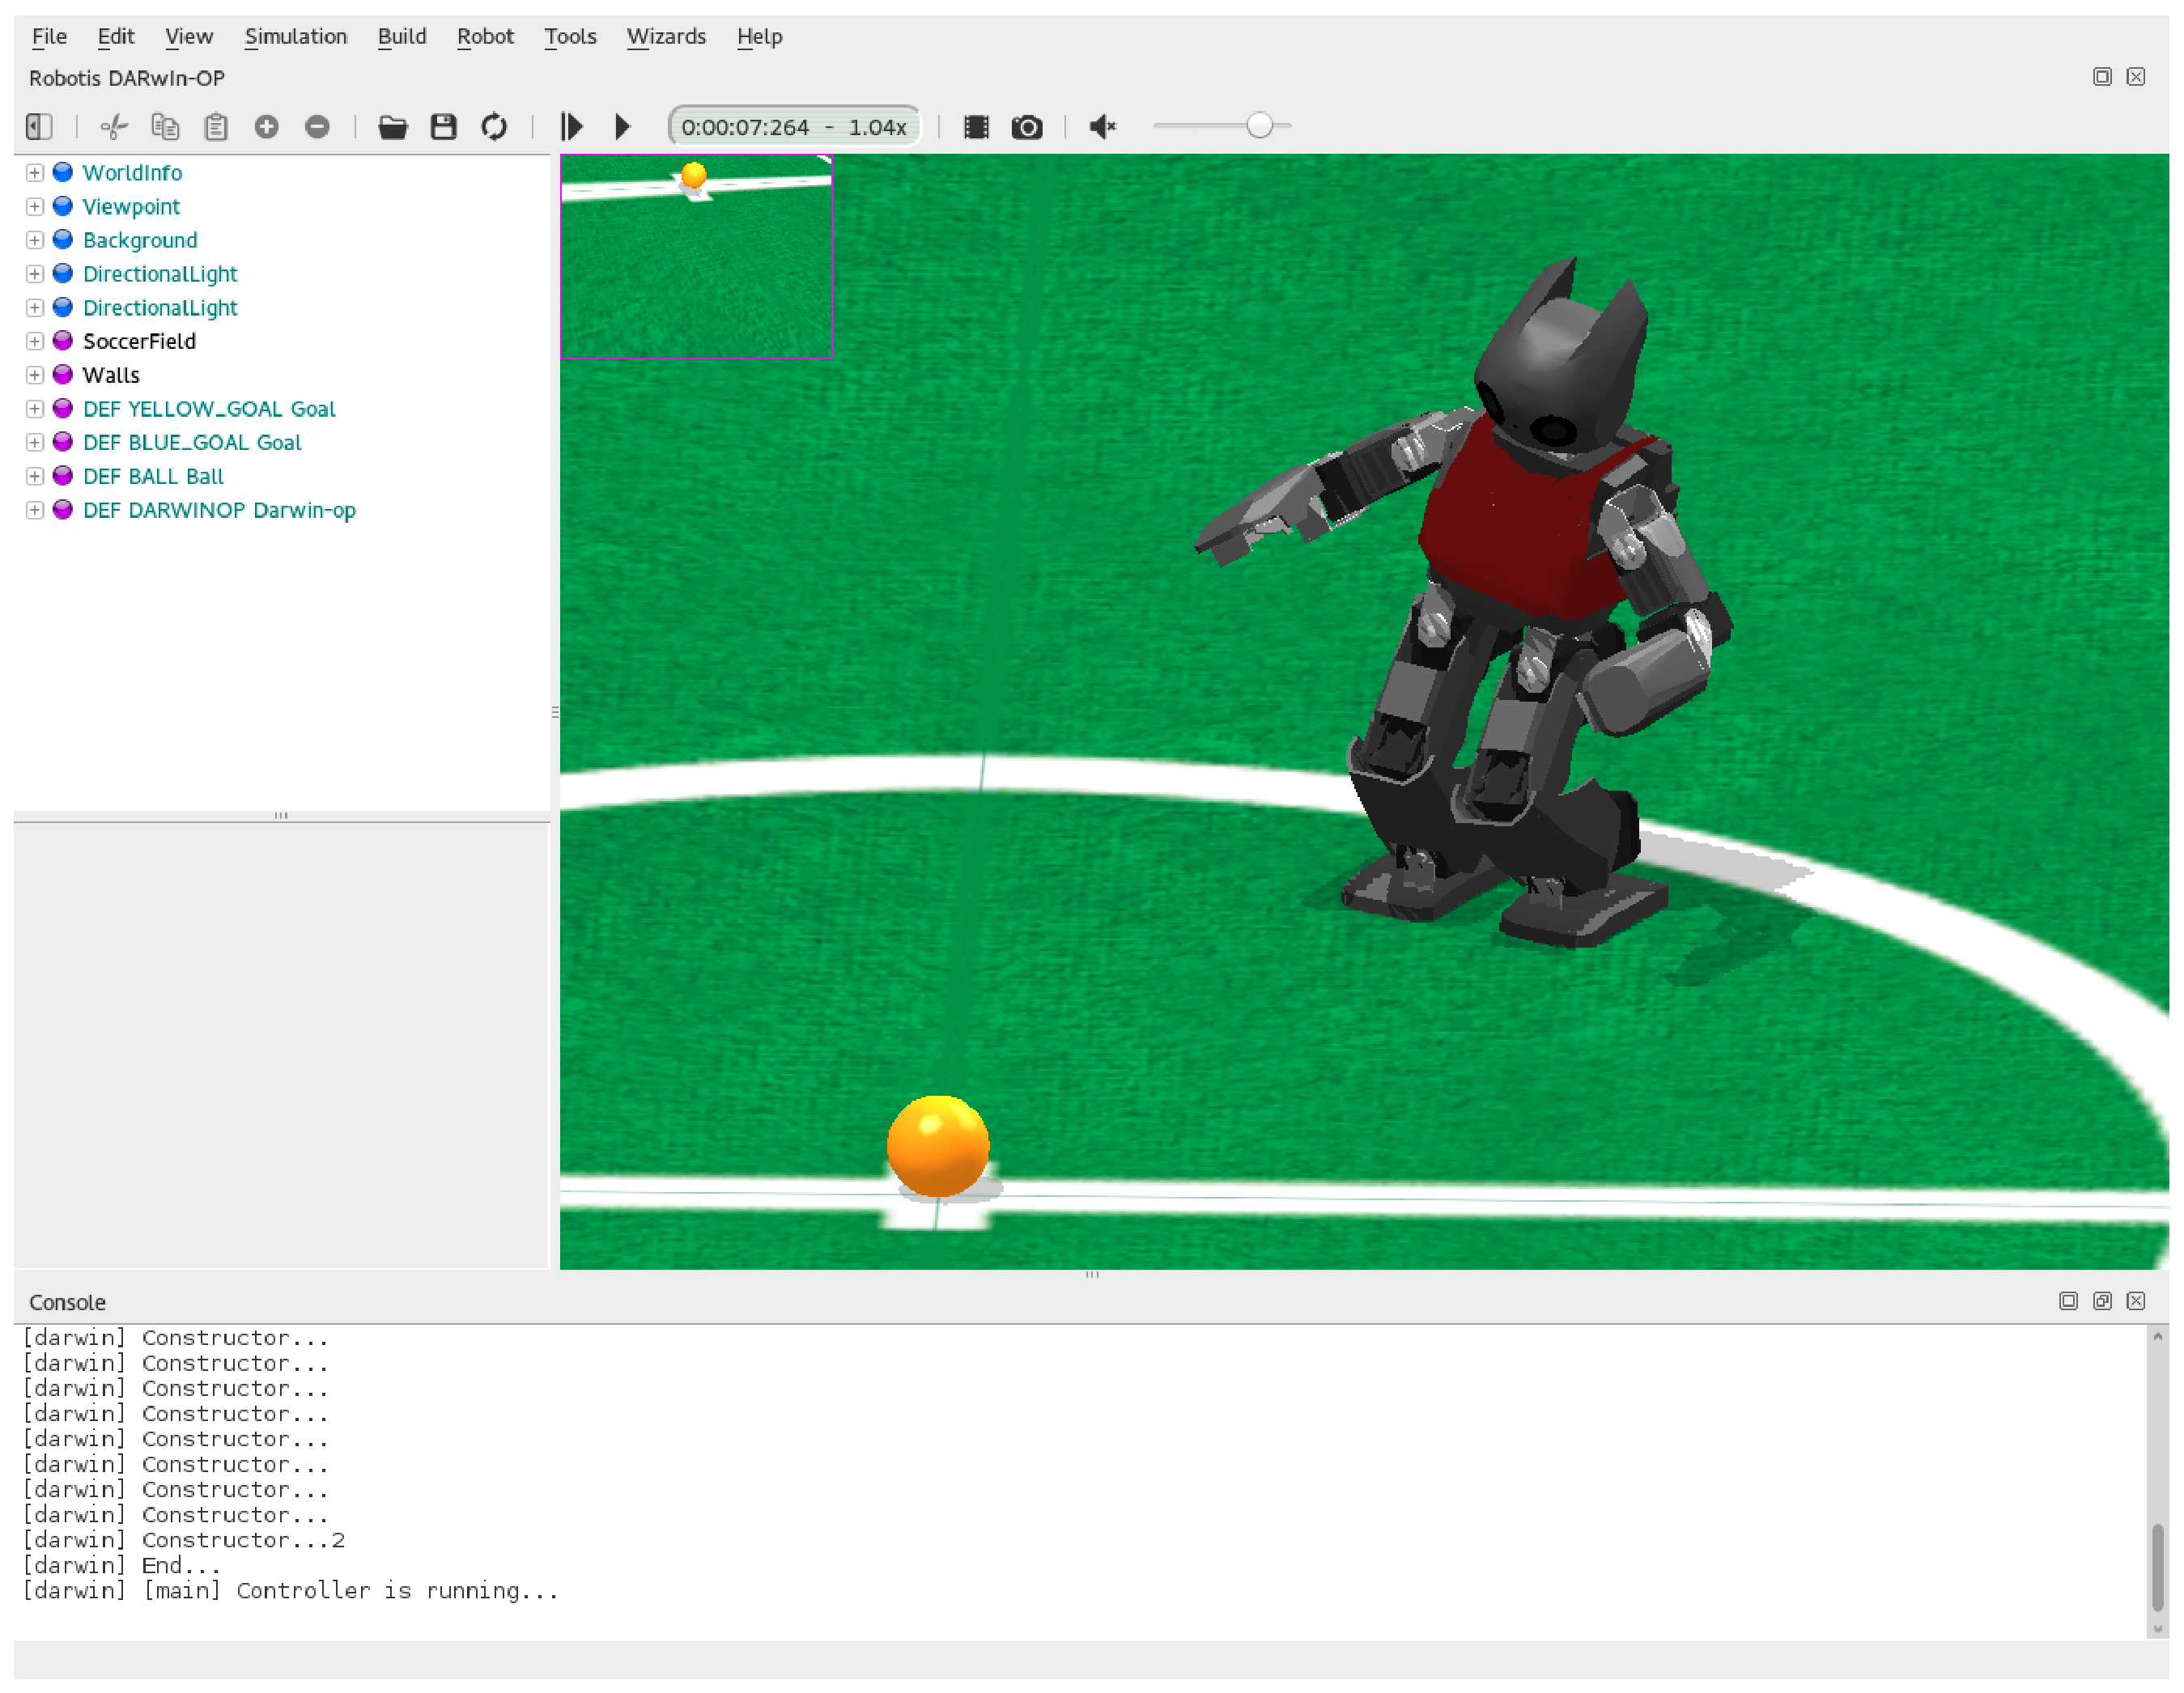
\includegraphics[width=1\linewidth]{1_webots_sample_window}}
\caption{Окно симулятора Webots.}
\label{im:1_webots_sample_window}
\end{figure}

Для запуска пользовательского контроллера на симулируемой модели робота требуется заранее произвести компиляцию программы с помощью Makefile и утилиты make. Образец Makefile был взят из демонстрационного контроллера Soccer. Так же каждый отдельный контроллер должен находиться в отдельном каталоге. Это требуется для того, чтобы симулятор мог найти бинарные файлы контроллера. Название каталога должно соответствовать названию бинарного файла. Выбрать контроллер можно с помощью соответственного пункта в меню (слева в окне симуляции) у объекта "DEF DARWINOP Darwin-OP".

Так же симулятор позволяет добавлять другие экземпляры робота на отображаемую сцену и запускать на нем отдельные требуемые реализации контроллера. Это позволят проводить тестирование поведения одновременно на нескольких роботах.

В Webots была замечена недокументированная особенность в поведении перенаправления данных со стандартного потока вывода в консоль симулятора. Данная консоль перенаправляет данные, полученные со стандартного потока вывода работающего контроллера. Отображение данных происходит только после получения символа конца строки (ASCII код соответствует значению 0A в шестнадцатеричной системе счисления). Другими словами выведенная строка не будет отображена без символа конца строки.

Для отладки исходного кода возможно использовать утилиту gdb. Данная утилита является отладчиком многих языков программирования на различных платформах с открытым исходным кодом. В данной работе для компиляции исходного кода используется компилятор gcc версии 5.1, доступный в официальном репозитории операционной системы ArchLinux. Для поддержки отладки требуется добавить флаг $-g$ при запуске компилятора.  Для этого достатачно в Makefile требуемого контроллера написать следующие строки:

\lstset{language=[gnu] make}
\begin{lstlisting}
CFLAGS = -g
\end{lstlisting}

Данная строка добавит соответствующий флаг компиляции при сборке проекта. Для сборки проекта с помощью Makefile используется утилита make. Эта утилита автоматизирует процесс преобразования файлов из одной формы в другую. В данной работе в Makefile описан процесс сборки исходного кода проекта. Подробное описание использования утилиты можно получить в официальной догументации и выходит за рамки работы \cite{stallman2006gnu}.

Для подключения утилиты отладки в системной командной строке требуется произвести запуск gdb и выполнить команду attach к PID (идентификатор процесса) запущенного контроллера. Идентификатор процесса можно получить из утилиты gnome-system-monitor или из любого другого аналогичного приложения. В данной работе процесс отладки подробно рассматриваться не будет. Более полную информацию можно получить из официальной документации утилиты gdb \cite{stallman1992gdb}.

Так же симулятор позволяет запускать контроллер для Darwin-OP на реальной модели робота (Рис. \ref{im:1_webots_transfer}) и получать информацию с устройств робота (Рис. \ref{im:1_webots_position_sensors}).

\begin{figure}[h]
\center{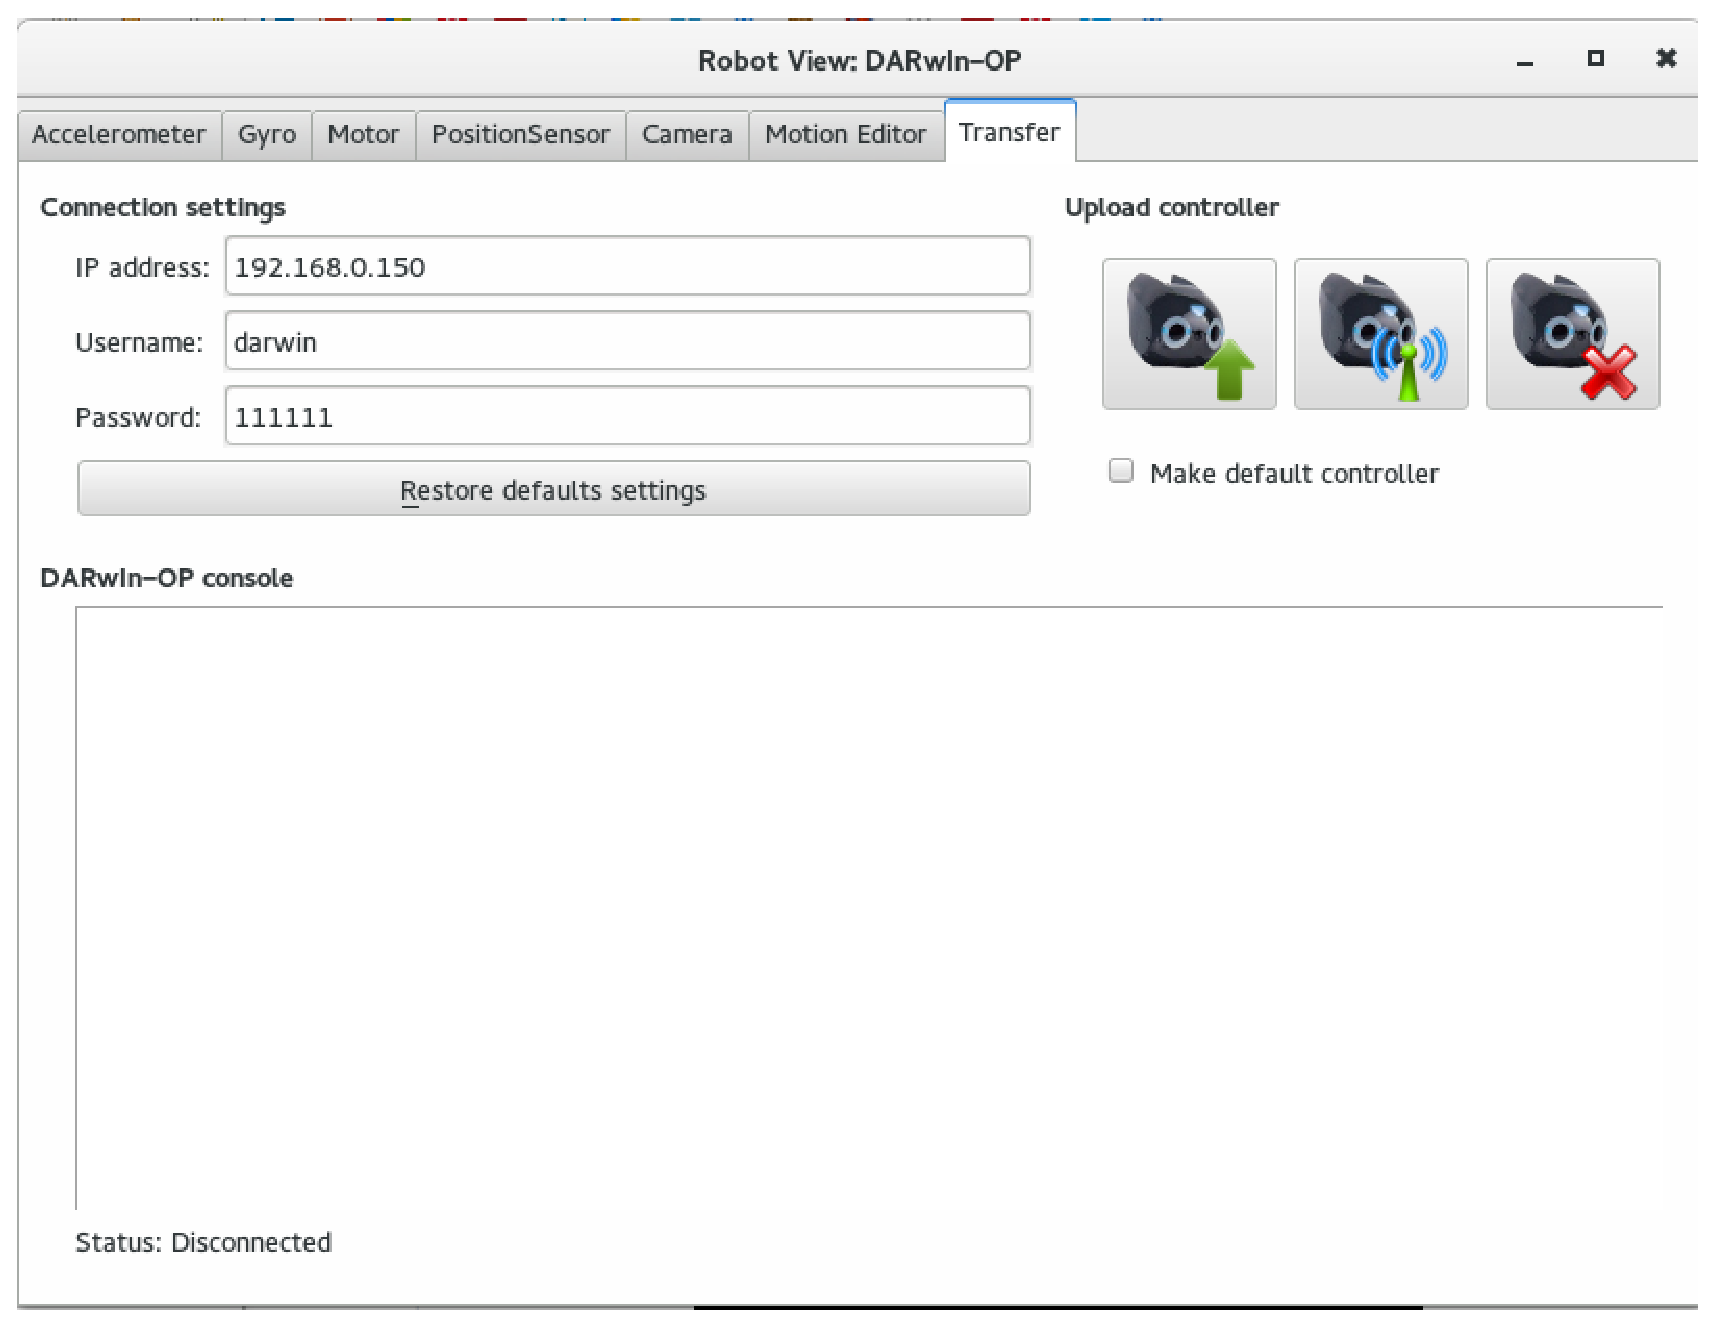
\includegraphics[width=1\linewidth]{1_webots_transfer}}
\caption{Окно запуска контроллера на реальном роботе.}
\label{im:1_webots_transfer}
\end{figure}

\begin{figure}[h]
\center{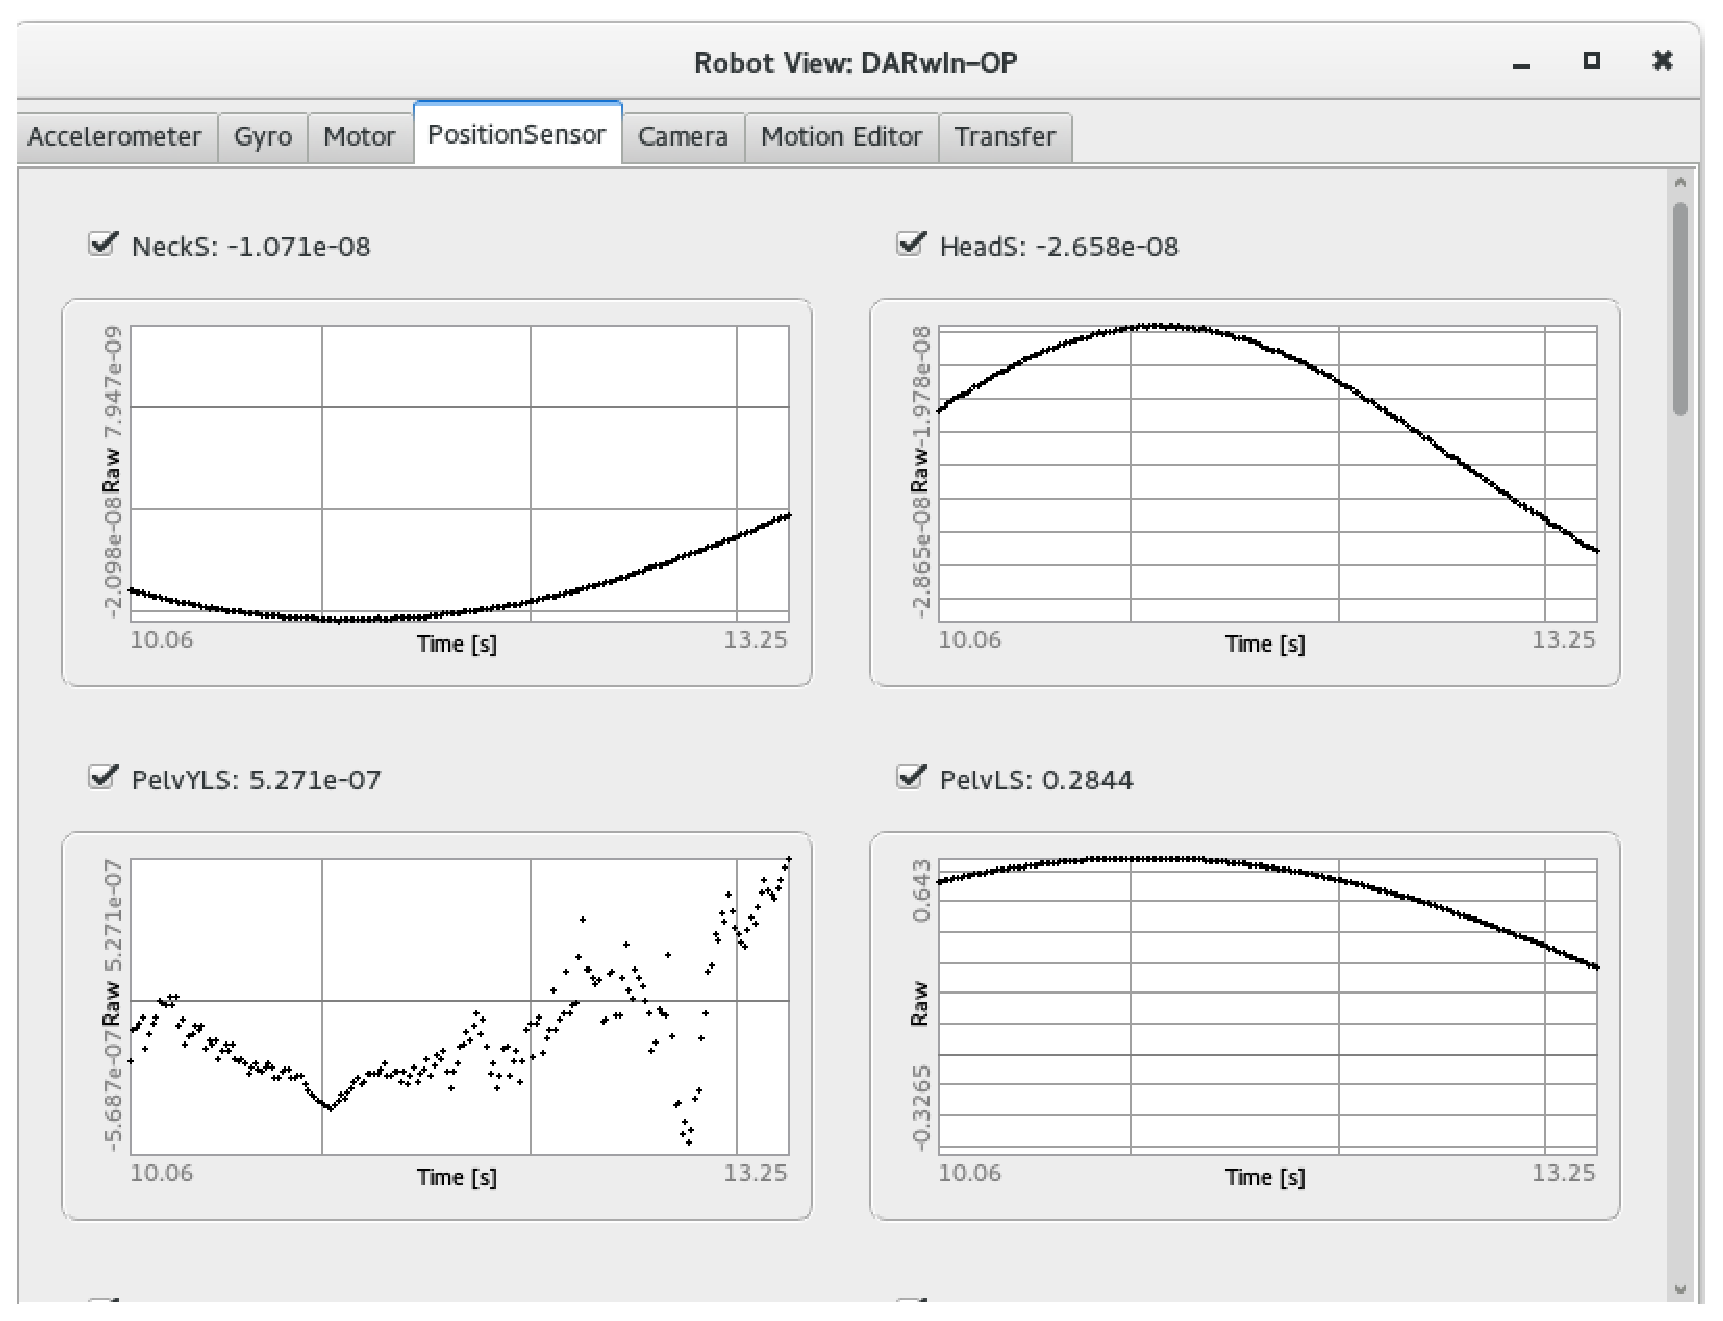
\includegraphics[width=1\linewidth]{1_webots_position_sensors}}
\caption{Показания позиционных сенсоров при выполнении движения.}
\label{im:1_webots_position_sensors}
\end{figure}


Подключение к роботу происходит по ssh протоколу. Этот протокол позволяет производить удаленное управление операционной системой через сетевое соединение. Подробное описание протокола не входит в цели данной работы. При первом подключении симулятора к реальному роботу происходит копирование исходного кода контроллера и библиотек Webots в соответствующий каталог во внутреннем диске робота. Далее происходит компиляция требуемых компонентов. Данные о процессе сборки выводятся в консоль диалогового окна. При успешном завершении процесса сборки требуемый контроллер сразу же запускается на роботе. Если контроллер не был запущен, то данный процесс должен быть запущен вручную через ssh соединение вне симулятора. Причина, по контроллер может не запуститься автоматически, не была установлена.

%### Изменения Makefile

Для возможности компиляции проекта, исходный код которого находится в разных подкаталогах корневой директории проекта, требуется внести некоторые изменения в Makefile на роботе, который находится в родительском каталоге директории с исходным кодом. Детально это будет рассмотрено в другой части работы. Стоит отметить, что данный файл необходимо редактировать после компиляции основных компонентов Webots на роботе, так как симулятор копирует данный файл из неизвестного источника при первом запуске на роботе. Данный факт был обнаружен экспериментальным путем и ранее никак не документирован.

В ходе анализа симуляционной Webots было получено общее представление о возможностях управления механикой робота. Webots API позволяет инициализировать Darwin Framework и упрощает процесс программного взаимодействия с устройствами робота. Так же анализ дал представление о методе реализации переносимого кода между симуляционной средой и реальным роботом.

\section{Анализ NAO SDK}

В данном разделе проведен обзор основного компонента управления сервоприводами робота из NAO SDK v.2.1. В данном компоненте имеются некоторые ключевые особенности, которые использованы в данной работе при разработке интерфейса класса управления механикой для Darwin-OP. Подробное описание комплекта средств разработки выходит за рамки данной работы и далее не рассматривается.

Управление моторами на роботе Aldebaran NAO происходит с помощью класса ALMotionProxy \cite{urlalmotion}. Данный класс предоставляет довольно обширный набор механизмов управления роботом. Так же данный класс позволяет управлять роботом по сети, когда контроллер запущен на удаленном компьютере, а не на самом роботе. Для увеличения производительности и упрощения архитектуры программного компонента в разрабатываемой библиотеке поддержка сетевого взаимодействия не будет реализована. В дальнейшем поддержка сети может быть реализована введением дополнительного дочернего класса с соответствующим интерфейсом управления, но проектирование данного класса не является основной целью данной работы.

Методы класса ALMotionProxy можно разбить на группы по способу управления. Все группы методов не будут рассматриваться в данном разделе. В данной работе интерес предоставляют только группы низкоуровнего управления механикой робота. Далее будут рассмотрены группы методов, которые имеют тесную взаимосвязь с интерфейсом разработанного класса для Darwin-op.

Самым примитивным способом управления роботом является управление его механикой напрямую с его сервоприводами (Joint control).  ALMotionProxy предоставляет набор методов, который позволяет задавать состояние мотора напрямую, либо изменять его значение относительно текущего положения. На вход функций подается список с именами моторов, на которых надо изменить значения, и список чисел с плавающей точкой, значения которых устанавливаются на моторы. Так же в качестве аргументов передается список с длинами временных интервалов, через которые значения углов будут установлены на конкретный привод.

Так же поддерживается управление частями тела в декартовой системе координат. На вход методам, управляющих частями тела робота в декартовой системе координат, по аналогии с ранее описанными функциями, передается вектор с названиями частей тела, значения, которые требуется установить, и длины временных интервалов, через которые будут установлены данные значения.

В этих методах управления можно обратить внимание на то, что обращение к изменяемым значениям происходит через обращение к параметру по его имени. Этот подход позволяет изменять схему управления без фактического изменения кода интерфейса.

В системе так же реализован способ управления походкой (Locomotion control). Она позволяет задать передвижение робота с постоянной скоростью и движение в определенную точку навигационной плоскости, относительно текущего положения. Данная группа движений не была реализована в основном классе управления механикой, разработанного в данной работе, по причине того, что эта группа не является низкоуровневым элементом управления движения робота. Данный способ управления следует вынести в отдельный класс, который описывает сложные движения и взаимодействует с низкоуровневым механизмом.

Анализ показал, что ALMotionProxy имеет обширное множество методов взаимодействия с роботом. Часть методов относится к высокоуровневым механизмам управления и следовало бы вынести в отдельные классы. Из данного класса была взята структура методов управления частями тела и отдельными моторами при реализации собственной библиотеки управления.